\subsection{Выбор и сравнение языковых моделей}
В процессе разработки диалогового агента для ролевых игр одним из ключевых решений стал выбор языковой модели, которая обеспечила бы оптимальный баланс между качеством генерации текста, быстродействием и возможностью локального запуска. Ориентация на локальные модели была продиктована следующими практическими соображениями:
\begin{itemize}
\item необходимость полного контроля над обработкой пользовательских данных;
\item отсутствие зависимости от внешних API и связанных с ними ограничений;
\item возможность тонкой настройки параметров инференса;
\item снижение эксплуатационных расходов при масштабировании проекта;
\item стабильность работы независимо от внешних сервисов.
\end{itemize}

Для разработки и тестирования использовалась видеокарта NVIDIA A100, предоставленная компанией МТС, что позволило эффективно работать с вычислительно-требовательными моделями. Рассматривались несколько высокопроизводительных моделей, способных работать на данном оборудовании: QwQ-32B, DeepSeek-R1-Distill-Qwen-32B, а также Falcon-40B \cite{reddit_a100}. Эти модели представляют собой современные языковые системы с различными архитектурными особенностями, размерами и характеристиками, что делает их сравнительный анализ важным этапом проектирования диалоговой системы для ролевых игр.
\subsubsection{Подход к выбору моделей}

При отборе языковых моделей для системы был применен многофакторный подход, учитывающий как технические возможности оборудования, так и специфические требования ролевой игры. Основные критерии оценки включали:

\begin{itemize}
\item \textbf{Качество генерации текста} — способность модели создавать связные, тематически релевантные ответы, соответствующие сеттингу древнего мира;
\item \textbf{Скорость инференса} — время отклика модели при генерации ответов, критически важное для поддержания естественного темпа диалога;
\item \textbf{Способность к поддержанию контекста} — умение модели сохранять последовательность в рамках продолжительной беседы;
\item \textbf{Понимание игровых сценариев} — корректная интерпретация запросов, связанных с военно-политическими событиями, социальными явлениями и государственным устройством;
\item \textbf{Устойчивость к нестандартным запросам} — адекватная реакция на провокационные вопросы и попытки выхода за рамки роли;
\item \textbf{Языковое разнообразие} — богатство лексики и стилистических приёмов при описании вымышленных государств, религий и культур.
\end{itemize}

Для объективного сравнения был разработан набор тестовых сценариев, моделирующих типичные ситуации в игре: создание новых государств, генерация событий (позитивных и негативных), описание культурных и религиозных особенностей. Все модели тестировались на одном и том же оборудовании (NVIDIA A100) для обеспечения сопоставимости результатов по скорости обработки запросов.
\subsubsection{Экспериментальное сравнение}

В рамках исследования было проведено сравнительное тестирование трех перспективных языковых моделей: QwQ-32B, DeepSeek-R1-Distill-Qwen-32B и Falcon-40B. Все модели были протестированы на идентичном наборе сценариев, отражающих ключевые аспекты игрового процесса в сеттинге древнего мира.

Результаты сравнения представлены в таблице, где оценки выставлялись по пятибалльной шкале:

\begin{table}[h]
\centering
\caption{Сравнительная оценка языковых моделей}
\label{tab:compare_models}
\begin{tabular}{|l|c|c|c|}
\hline
\textbf{Критерий} & \textbf{QwQ-32B} & \textbf{DeepSeek-32B} & \textbf{Falcon-40B} \\
\hline
Качество & 4 & 4.5 & 1 \\
\hline
Скорость & 3 & 5 & 2 \\
\hline
Поддержание & 3.5 & 4 & 1 \\
\hline
Понимание & 4 & 4 & 1 \\
\hline
Устойчивость & 2 & 4 & 1 \\
\hline
Разнообразие & 4 & 4 & 1 \\
\hline
Русский & \textbf{0} & \textbf{4} & \textbf{3} \\
\hline
\textbf{Сумма} & \textbf{20.5} & \textbf{29.5} & \textbf{10} \\
\hline
\end{tabular}
\end{table}


Как видно из результатов, модель DeepSeek-R1-Distill-Qwen-32B продемонстрировала наилучшие показатели по большинству критериев, особенно выделяясь по скорости инференса, качеству генерации и поддержке русского языка. Модель QwQ-32B показала хорошие результаты на английском языке, особенно в плане языкового разнообразия и понимания игровых сценариев, но практически не поддерживала русский язык, что критически важно для целевой аудитории проекта. Модель Falcon-40B показала неудовлетворительные результаты по всем параметрам, не справившись с базовыми игровыми сценариями.

Полные протоколы тестирования с примерами ответов моделей на различные запросы представлены в Приложении \ref{appendix:3}, что позволяет получить более детальное представление о качественных различиях между моделями.

\subsection{Архитектура и ключевые компоненты}
Разработанная система представляет собой комплексное программное решение, объединяющее языковую модель, асинхронные обработчики запросов и интерфейс мессенджера для создания интерактивного игрового мира. Архитектура проекта построена на принципах асинхронности, что позволяет обрабатывать запросы от множества пользователей одновременно без блокировки основного потока выполнения. Каждый компонент системы выполняет строго определённую функцию, а состояние игроков и игрового мира надёжно сохраняется в базе данных, обеспечивая персистентность и целостность игрового процесса между сессиями. Ключевая особенность реализации заключается в эффективной организации взаимодействия между пользовательским интерфейсом в Telegram, механизмом извлечения релевантной информации (RAG) и языковой моделью DeepSeek, обеспечивающей генерацию контекстно-зависимых ответов с учётом истории государства, особенностей мира и текущих игровых событий.
\subsubsection{Схема взаимодействия компонентов}

Архитектура системы построена на основе модульного подхода с чёткой сегментацией ответственности между компонентами. Общая схема взаимодействия элементов представлена на рисунке \ref{fig:flowchart}.

\begin{figure}[h]
    \centering
    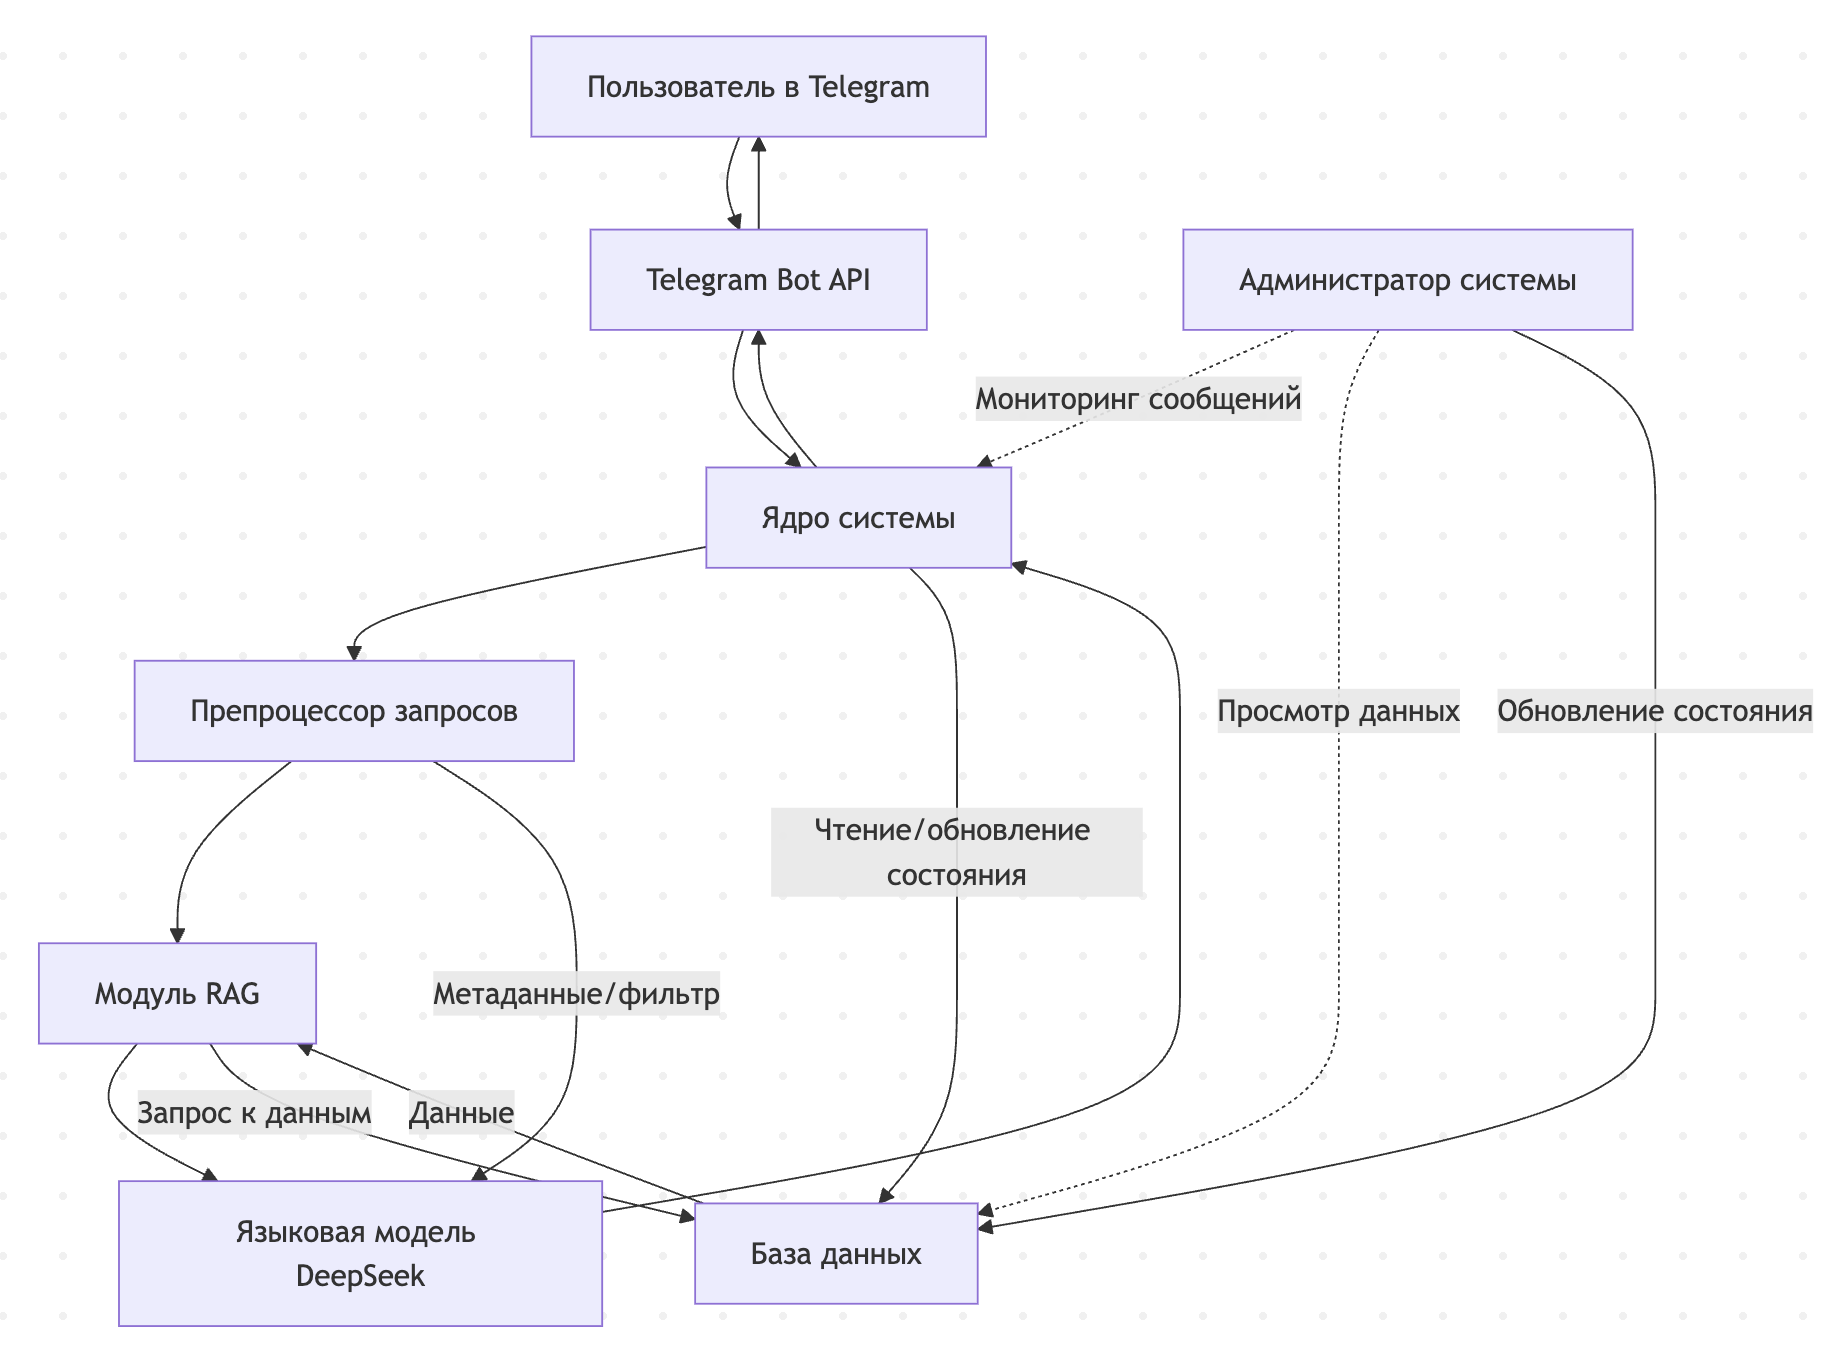
\includegraphics[width=0.8\textwidth]{figures/flowchart}
    \caption{Архитектура системы и взаимодействие компонентов}
    \label{fig:flowchart}
\end{figure}\\
~\\~\\~\\~\\~\\

Центральным звеном архитектуры выступает ядро системы, координирующее взаимодействие между всеми компонентами. Поток данных начинается с пользовательского интерфейса в Telegram, где игроки отправляют сообщения и команды. Telegram Bot API транслирует эти запросы в асинхронный обработчик сообщений, который определяет тип запроса и маршрутизирует его в соответствующий функциональный модуль.

Для обработки игровых взаимодействий задействуется цепочка компонентов:

\begin{itemize}
\item \textbf{Препроцессор запросов} анализирует входящие сообщения, фильтрует запрещенные термины и подготавливает контекст для языковой модели.

\item \textbf{Модуль RAG (Retrieval-Augmented Generation)} извлекает из базы данных релевантную информацию об игровом мире, стране игрока и исторических событиях, обогащая контекст запроса.

\item \textbf{Языковая модель DeepSeek} генерирует ответы на основе обогащенного контекста, сохраняя согласованность с игровым миром и стилистическую уместность.

\item \textbf{База данных} хранит информацию о пользователях, странах, игровых событиях и истории взаимодействий, обеспечивая персистентность игрового мира.
\end{itemize}

Асинхронная природа системы позволяет обрабатывать запросы от множества игроков одновременно, не блокируя основной поток выполнения. Каждый запрос обрабатывается в отдельной задаче, что оптимизирует использование ресурсов и повышает отзывчивость системы.

Для администраторов реализован отдельный интерфейс управления, позволяющий мониторить состояние системы, вносить коррективы в игровой мир и разрешать возникающие конфликтные ситуации без прерывания игрового процесса для остальных пользователей.

\subsubsection{RAG-модуль (Retrieval-Augmented Generation)}

\subsubsection{Обработка пользовательских запросов и генерация ответов}

\subsubsection{Регистрация и учёт игроков}

\subsubsection{Интеграция с Telegram}

\subsection{Проверка соответствия ответов бота требованиям}
\subsubsection{Критерии качества игровых ответов и ролевого поведения}
\subsubsection{Тестирование на антураж и отсутствие современных терминов}
\subsubsection{Типовые диалоги и анализ релевантности}
\subsubsection{Системы фильтрации и самоконтроля}

\subsection{Обратная связь и оценки пользователей}
\subsubsection{Организация раннего тестирования}
\subsubsection{Описание отзывов тестовых игроков}
\subsubsection{Изменения в системе по результатам обратной связи}

\subsection{Результаты и итоговая спецификация}
\subsubsection{Функциональные возможности финальной версии}
\subsubsection{Ограничения и известные проблемы}
\subsubsection{Перспективы дальнейшего развития}